
\chapter{Instalace}

\noindent
Defaultně potřebuje aplikace porty 4500 (server rozpoznávající SPZ), 8080 (backend) a
8889 (frontend). Pokud je MongoDB instalována systémově, běží na portu 27017, a pokud
v Dockeru, tak běží na portu 5432.
Porty lze změnit v konfiguračních souborech jednotlivých
komponent. Při změně portu komponenty A, na které jsou jiné komponenty B závislé,
je potřeba změnit port závislých komponent B pro danou komponentu A.
Mobilní aplikace se kompiluje vývojovým prostředím Android Studio.

\section{Soubory nastavení}

\noindent
Soubory pro nastavení jsou:

\begin{itemize}
  \setlength\itemsep{-.3em}
  \item Backend
  \begin{itemize}
    \item /backend/Dockerfile
    \item /backend/config/production.json
    \item /backend/config/development.json
    \item /backend/src/config.ts
  \end{itemize}
  \item Frontend
  \begin{itemize}
    \item /frontend/Dockerfile
    \item /frontend/config/main.js
    \item /frontend/config/main.local.js
  \end{itemize}
  \item Server rozpoznávající SPZ
  \begin{itemize}
    \item /express-openalpr-server/Dockerfile
    \item /express-openalpr-server/processes.json
  \end{itemize}
\end{itemize}

\newpage
\section{Instalace Dockerem}

\noindent
Instalace celého systému Dockerem je velice jednoduchá, ten zajistí kompilaci,
spuštění, propojení všech částí a odhalení potřebných služeb ven na internet. \citep[][]{DockerDocs}

% Kromě Backendu, Frontendu, OpenALPR Server a MongoDB používá tato distribuce
% Dockerem populární HTTP server NGINX pro SSL a reverse proxy. Vnitřní HTTP komunikace
% tak nemusí být zabezpečena.

\subsubsection*{Postup instalace}

\begin{enumerate}
  \setlength\itemsep{.05em}
  \item Po stažení git repozitáře se zdrojovým kódem nastavíme submoduly (lze vynechat, pokud máte kód jako zip archiv):\\
  \begin{lstlisting}[numbers=none]
    $ git submodule init
    $ git submodule update --remote --recursive
  \end{lstlisting}
  \item Dle potřeby upravíme soubor \textit{/docker-compose.yml} a ostatní konfigurační soubory.
  \item Celý systém spustíme.\\
  \begin{lstlisting}[numbers=none]
    $ docker-compose up
  \end{lstlisting}
  \item Zjistíme počáteční přihlašovací údaje z výstupu předchozího příkazu. Pokud byla proměnná prostředí \texttt{NODE\_ENV=development},
  bude počátečení heslo 1234.\\\\
  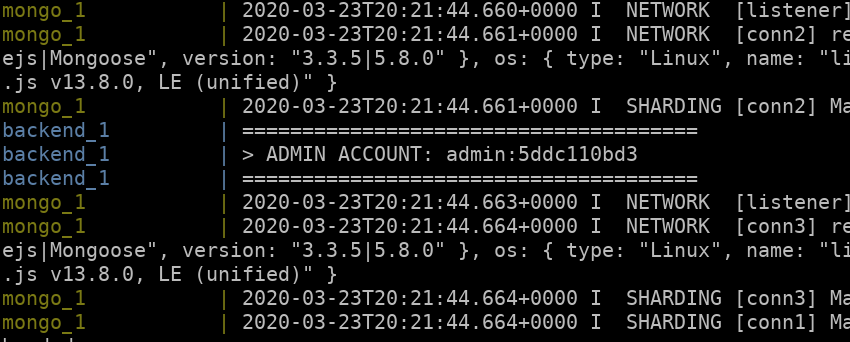
\includegraphics[width=100mm]{../img/installation_pass.png}\\
  \item Otevřeme prohlížeč na adrese \url{http://localhost:8889}.
\end{enumerate}

Krok číslo 3 může trvat i několik minut v závislosti na rychlosti internetového
přípojení. Protože Docker zabalí vše včetně systémových závislostí, velikost
výsledných imagů je kolem $1,4$GB.

Pro detaily je potřeba konzultovat soubor \textit{/docker-compose.yml}, jednotlivé soubory
zvané \textit{Dockerfile} každé komponenty a konfigurační soubory komponent.

\section{Instalace bez Dockeru}

\noindent
Pro spuštění bez Dockeru je potřeba nainstalovat několik programů. Jmenovitě se
jedná o Typescript pro kompilaci, Node.js a NPM pro knihovny a spuštění backendu, frontendu
a serveru rozpoznávající SPZ, pm2 pro load-balancing serveru rozpoznávající SPZ, MongoDB,
Android Studio pro kompilaci mobilní aplikace a pro rozpoznávání SPZ je potřeba OpenALPR .

Instalace knihovny OpenALPR je nejproblematičtější, protože
probíhá kompilací velkého množství C++. Instrukce ke kompilaci
jsou dostupné z \url{https://github.com/openalpr/openalpr#compiling}. Další alternativou je spouštet server rozpoznávající SPZ
Dockerem a zbytek bez Dockeru -- stačí ve složce \textit{/express-openalpr-server} spustit příkazy: \textbf{asddddddddddddddddddddddddddddd}

\begin{lstlisting}[numbers=none]
  $ npm install
  $ docker build -t express-openalpr:latest "."
  $ docker run express-openalpr:latest 
\end{lstlisting}

\subsubsection*{Postup spuštění bez Dockeru}

\begin{enumerate}
  \setlength\itemsep{.05em}
  \item Nainstalujeme závislosti.
  \item Po stažení git repozitáře se zdrojovým kódem nastavíme submoduly (lze vynechat, pokud máte kód jako zip archiv):\\
  \begin{lstlisting}[numbers=none]
    $ git submodule init
    $ git submodule update --remote --recursive
  \end{lstlisting}
  \item Spustíme MongoDB.
  \item Spustíme server rozpoznávající SPZ.\\
  \begin{lstlisting}[numbers=none]
    $ cd express-openalpr-server
    $ npm install
    $ pm2 start processes.json
  \end{lstlisting}
  \item Spustíme backend buď následujícími příkazy, nebo bash skriptem \textit{/backend/sdev.sh -c}.\\
  \begin{lstlisting}[numbers=none]
    $ cd backend
    $ npm install
    $ npm run compile
    $ npm start
  \end{lstlisting}
  \item Spustíme frontend (poslední příkaz může chvíli trvat).\\
  \begin{lstlisting}[numbers=none]
    $ cd frontend
    $ npm install
    $ npm start
  \end{lstlisting}
  \item Přihlašovací údaje jsou \texttt{admin:1234}, protože nespouštíme s proměnnou prostředí \texttt{NODE\_ENV=production} jako při spuštění Dockerem.
  \item Otevřeme prohlížeč na adrese \url{http://localhost:8889}.
\end{enumerate}
